\chapter{Resultados}

A continuación, se presentan los resultados obtenidos a partir de las 34
pruebas realizadas con el prototipo. Para cada participante se dispone de
un registro generado automáticamente por el sistema durante la 
experiencia y de una encuesta posterior. Los registros contienen 
información sobre las interacciones realizadas, el desempeño en los 
minijuegos, los estados asignados al jugador y los cambios de dificultad
efectuados durante la sesión. Por su parte, la encuesta contiene las 
respuestas relacionadas con dificultad e interacción, incluyendo
atención a la canción, diversión, sensación de agobio, desempeño 
percibido y minijuego señalado como más frustrante.

\section{Resultados de telemetría}
Los archivos de métricas registran las interacciones realizadas durante 
cada sesión y permiten agrupar los datos según participante, minijuego y
la hora exacta en la que ocurrió. Para cada actividad se presentan los
resultados relacionados con aciertos, fallos, omisiones y las métricas 
específicas disponibles para cada tipo de interacción. Debido a que no 
todos los minijuegos utilizan las mismas variables de precisión o tiempo, 
los indicadores generales se presentan de forma conjunta y las métricas 
específicas se reportan únicamente para las actividades en las que son 
registradas por el sistema.

% Resultados globales de las interacciones registradas por minijuego.
\begin{table}[H]
    \centering
    \caption{Resultados globales de las interacciones registradas por minijuego.}
    \label{tab:resultadosGlobales}

    \renewcommand{\arraystretch}{1.3}
    \setlength{\tabcolsep}{4pt}

    \begin{tabularx}{\textwidth}{
        |>{\centering\arraybackslash}X
        |>{\centering\arraybackslash}X
        |>{\centering\arraybackslash}X
        |>{\centering\arraybackslash}X
        |>{\centering\arraybackslash}X
        |>{\centering\arraybackslash}X|
    }
        \hline

        \textbf{Minijuego} &
        \textbf{Aciertos} &
        \textbf{Errores} &
        \textbf{Omisiones} &
        \textbf{Total interacciones} &
        \textbf{Tasa de éxito} \\ \hline

        Alex & 1558 & 322 & 514 & 2394 & 65.08\% \\ \hline
        Joaquin & 423 & 172 & 0 & 595 & 71.09\% \\ \hline
        Shipi & 262 & 270 & 22 & 554 & 47.29\% \\ \hline
        Juan Andres & 208 & 304 & 69 & 581 & 35.80\% \\ \hline
        Danniel & 326 & 245 & 31 & 602 & 54.15\% \\ \hline
        Jeremy & 195 & 95 & 32 & 322 & 60.56\% \\ \hline

    \end{tabularx}
\end{table}

% Mediana del error de timing promedio de los participantes por minijuego.
\begin{table}[H]
    \centering
    \caption{Mediana del error de timing promedio de los participantes por minijuego.}
    \label{tab:errorTimingMinijuegos}

    \small
    \renewcommand{\arraystretch}{1.3}
    \setlength{\tabcolsep}{4pt}

    \begin{tabularx}{\textwidth}{
        |>{\centering\arraybackslash}X
        |>{\centering\arraybackslash}X|
    }
        \hline

        \textbf{Minijuego} &
        \textbf{Mediana del error promedio (s)} \\ \hline

        Alex & 0.018 \\ \hline
        Joaquin & 0.095 \\ \hline
        Shipi & 0.435 \\ \hline
        Juan Andres & 1.045 \\ \hline
        Danniel & 0.098 \\ \hline
        Jeremy & 0.126 \\ \hline

    \end{tabularx}
\end{table}

% Promedio de las métricas específicas de interacción registradas en los 
% minijuegos Shipi, Juan Andres y Jeremy.
\begin{table}[H]
    \centering
    \caption{Promedio de las métricas específicas de interacción registradas en los minijuegos Shipi, Juan Andres y Jeremy.}
    \label{tab:metricasEspecificas}

    \small
    \renewcommand{\arraystretch}{1.3}
    \setlength{\tabcolsep}{4pt}

    \begin{tabularx}{\textwidth}{
        |>{\centering\arraybackslash}X
        |>{\centering\arraybackslash}X
        |>{\centering\arraybackslash}X
        |>{\centering\arraybackslash}X|
    }
        \hline

        \textbf{Minijuego} &
        \textbf{Tiempo de reacción (s)} &
        \textbf{Precisión de dirección} &
        \textbf{Mano correcta (\%)} \\ \hline

        Shipi & 0.582 & 0.536 & --- \\ \hline
        Juan Andres & --- & 0.521 & 73.42\% \\ \hline
        Jeremy & --- & 0.712 & 92.98\% \\ \hline

    \end{tabularx}
\end{table}


\section{Comportamiento del sistema adaptativo}
Además de las interacciones, los registros almacenan los estados 
asignados al jugador y los cambios de dificultad realizados durante la 
ejecución. A continuación, se presentan la frecuencia de aparición de 
los estados registrados por el sistema y las modificaciones efectuadas 
entre los niveles de dificultad disponibles. Los resultados se agrupan 
por participante y minijuego para mostrar cuántas veces se registra cada 
estado y cuántas modificaciones de dificultad se producen durante la 
experiencia. También se indetifica la dirección de cada cambio, 
diferenciando los incrementos, reducciones y períodos en los que la 
dificultad permanece sin modificación.

% Cantidad de estados idle, engaged y overloaded registrados por 
% participante
\begin{table}[H]
    \centering
    \caption{Cantidad de estados \textit{idle}, \textit{engaged} y \textit{overloaded} registrados por participante.}
    \label{tab:cantidadEstados}

    \renewcommand{\arraystretch}{1.3}
    \setlength{\tabcolsep}{4pt}

    \begin{tabularx}{\textwidth}{
        |>{\centering\arraybackslash}X
        |>{\centering\arraybackslash}X
        |>{\centering\arraybackslash}X
        |>{\centering\arraybackslash}X
        |>{\centering\arraybackslash}X|
    }
        \hline
        \textbf{ID} &
        \textbf{\textit{Idle}} &
        \textbf{\textit{Engaged}} &
        \textbf{\textit{Overloaded}} &
        \textbf{Total} \\ \hline

        P001 & 8 & 12 & 7 & 27 \\ \hline
        P002 & 8 & 14 & 7 & 29 \\ \hline
        P003 & 5 & 11 & 10 & 26 \\ \hline
        P004 & 8 & 11 & 5 & 24 \\ \hline
        P005 & 7 & 9 & 4 & 20 \\ \hline
        P006 & 6 & 9 & 4 & 19 \\ \hline
        P007 & 6 & 10 & 6 & 22 \\ \hline
        P008 & 5 & 9 & 7 & 21 \\ \hline
        P010 & 8 & 11 & 5 & 24 \\ \hline
        P011 & 7 & 10 & 7 & 24 \\ \hline
        P012 & 4 & 10 & 7 & 21 \\ \hline
        P013 & 8 & 13 & 6 & 27 \\ \hline
        P014 & 7 & 10 & 5 & 22 \\ \hline
        P015 & 8 & 12 & 8 & 28 \\ \hline
        P016 & 8 & 11 & 5 & 24 \\ \hline
        P017 & 6 & 10 & 7 & 23 \\ \hline
        P018 & 6 & 11 & 7 & 24 \\ \hline
        P019 & 7 & 10 & 6 & 23 \\ \hline
        P020 & 9 & 12 & 6 & 27 \\ \hline
        P021 & 8 & 13 & 9 & 30 \\ \hline
        P022 & 7 & 11 & 6 & 24 \\ \hline
        P023 & 5 & 8 & 6 & 19 \\ \hline
        P024 & 5 & 8 & 4 & 17 \\ \hline
        P025 & 7 & 13 & 8 & 28 \\ \hline
        P026 & 6 & 9 & 5 & 20 \\ \hline
        P027 & 5 & 8 & 5 & 18 \\ \hline
        P028 & 7 & 9 & 7 & 23 \\ \hline
        P029 & 6 & 8 & 5 & 19 \\ \hline
        P030 & 9 & 14 & 6 & 29 \\ \hline
        P031 & 8 & 10 & 4 & 22 \\ \hline
        P032 & 4 & 10 & 8 & 22 \\ \hline
        P033 & 8 & 13 & 8 & 29 \\ \hline
        P034 & 4 & 7 & 5 & 16 \\ \hline
        P036 & 5 & 11 & 7 & 23 \\ \hline
    \end{tabularx}
\end{table}

% Cantidad de aumentos y disminuciones de dificultad registrados por 
% participante
\begin{table}[H]
    \centering
    \caption{Cantidad de aumentos y disminuciones de dificultad registrados por participante.}
    \label{tab:cambiosDificultad}

    \renewcommand{\arraystretch}{1.3}
    \setlength{\tabcolsep}{4pt}

    \begin{tabularx}{\textwidth}{
        |>{\centering\arraybackslash}X
        |>{\centering\arraybackslash}X
        |>{\centering\arraybackslash}X
        |>{\centering\arraybackslash}X|
    }
        \hline

        \textbf{ID} &
        \textbf{Aumento de dificultad} &
        \textbf{Disminución de dificultad} &
        \textbf{Cambios totales} \\ \hline

        P001 & 3 & 4 & 7 \\ \hline
        P002 & 5 & 6 & 11 \\ \hline
        P003 & 4 & 5 & 9 \\ \hline
        P004 & 4 & 4 & 8 \\ \hline
        P005 & 4 & 3 & 7 \\ \hline
        P006 & 4 & 4 & 8 \\ \hline
        P007 & 1 & 2 & 3 \\ \hline
        P008 & 1 & 2 & 3 \\ \hline
        P010 & 2 & 3 & 5 \\ \hline
        P011 & 3 & 4 & 7 \\ \hline
        P012 & 6 & 5 & 11 \\ \hline
        P013 & 5 & 6 & 11 \\ \hline
        P014 & 1 & 2 & 3 \\ \hline
        P015 & 3 & 4 & 7 \\ \hline
        P016 & 2 & 3 & 5 \\ \hline
        P017 & 2 & 3 & 5 \\ \hline
        P018 & 5 & 6 & 11 \\ \hline
        P019 & 2 & 3 & 5 \\ \hline
        P020 & 1 & 2 & 3 \\ \hline
        P021 & 5 & 6 & 11 \\ \hline
        P022 & 2 & 3 & 5 \\ \hline
        P023 & 1 & 2 & 3 \\ \hline
        P024 & 3 & 2 & 5 \\ \hline
        P025 & 5 & 6 & 11 \\ \hline
        P026 & 4 & 4 & 8 \\ \hline
        P027 & 1 & 2 & 3 \\ \hline
        P028 & 1 & 2 & 3 \\ \hline
        P029 & 1 & 2 & 3 \\ \hline
        P030 & 4 & 5 & 9 \\ \hline
        P031 & 1 & 2 & 3 \\ \hline
        P032 & 2 & 3 & 5 \\ \hline
        P033 & 3 & 4 & 7 \\ \hline
        P034 & 3 & 4 & 7 \\ \hline
        P036 & 2 & 2 & 4 \\ \hline

    \end{tabularx}
\end{table}

% Mediana de las entradas a los estados del jugador y los ajustes de 
% dificultad registrados por participante en cada minijuego.
\begin{table}[H]
    \centering
    \caption{Mediana de las entradas a los estados del jugador y los ajustes de dificultad registrados por participante en cada minijuego.}
    \label{tab:estadosAjustesMinijuegos}

    \small
    \renewcommand{\arraystretch}{1.3}
    \setlength{\tabcolsep}{4pt}

    \begin{tabularx}{\textwidth}{
        |>{\centering\arraybackslash}X
        |>{\centering\arraybackslash}X
        |>{\centering\arraybackslash}X
        |>{\centering\arraybackslash}X
        |>{\centering\arraybackslash}X|
    }
        \hline

        \textbf{Minijuego} &
        \textbf{Entradas a Engaged} &
        \textbf{Entradas a Overloaded} &
        \textbf{Aumentos de dificultad} &
        \textbf{Disminuciones de dificultad} \\ \hline

        Alex & 3.0 & 2.0 & 1.0 & 1.0 \\ \hline
        Joaquin & 1.0 & 0.0 & 1.0 & 0.0 \\ \hline
        Shipi & 2.0 & 1.0 & 0.0 & 1.0 \\ \hline
        Juan Andres & 1.0 & 1.0 & 0.0 & 0.0 \\ \hline
        Danniel & 2.0 & 1.0 & 0.0 & 0.0 \\ \hline
        Jeremy & 1.0 & 0.0 & 0.0 & 0.0 \\ \hline

    \end{tabularx}
\end{table}


% Cantidad de cambios entre cada dificultad por participante
\begin{table}[H]
    \centering
    \caption{Cantidad de cambios entre cada dificultad por participante.}
    \label{tab:cambiosPorDificultad}

    \renewcommand{\arraystretch}{1.3}
    \setlength{\tabcolsep}{4pt}

    \begin{tabularx}{\textwidth}{
        |>{\centering\arraybackslash}X
        |>{\centering\arraybackslash}X
        |>{\centering\arraybackslash}X
        |>{\centering\arraybackslash}X
        |>{\centering\arraybackslash}X|
    }
        \hline

        \textbf{ID} &
        \textbf{Fácil a normal} &
        \textbf{Normal a díficil} &
        \textbf{Díficil a normal} &
        \textbf{Normal a fácil} \\ \hline

        P001 & 2 & 1 & 1 & 3 \\ \hline
        P002 & 1 & 4 & 4 & 2 \\ \hline
        P003 & 0 & 4 & 4 & 1 \\ \hline
        P004 & 2 & 2 & 2 & 2 \\ \hline
        P005 & 1 & 3 & 2 & 1 \\ \hline
        P006 & 2 & 2 & 2 & 2 \\ \hline
        P007 & 1 & 0 & 0 & 2 \\ \hline
        P008 & 1 & 0 & 0 & 2 \\ \hline
        P010 & 2 & 0 & 0 & 3 \\ \hline
        P011 & 1 & 2 & 2 & 2 \\ \hline
        P012 & 2 & 4 & 3 & 2 \\ \hline
        P013 & 1 & 4 & 4 & 2 \\ \hline
        P014 & 1 & 0 & 0 & 2 \\ \hline
        P015 & 1 & 2 & 2 & 2 \\ \hline
        P016 & 2 & 0 & 0 & 3 \\ \hline
        P017 & 2 & 0 & 0 & 3 \\ \hline
        P018 & 2 & 3 & 3 & 3 \\ \hline
        P019 & 1 & 1 & 1 & 2 \\ \hline
        P020 & 1 & 0 & 0 & 2 \\ \hline
        P021 & 2 & 3 & 3 & 3 \\ \hline
        P022 & 0 & 2 & 2 & 1 \\ \hline
        P023 & 1 & 0 & 0 & 2 \\ \hline
        P024 & 1 & 2 & 1 & 1 \\ \hline
        P025 & 2 & 3 & 3 & 3 \\ \hline
        P026 & 1 & 3 & 3 & 1 \\ \hline
        P027 & 1 & 0 & 0 & 2 \\ \hline
        P028 & 1 & 0 & 0 & 2 \\ \hline
        P029 & 1 & 0 & 0 & 2 \\ \hline
        P030 & 2 & 2 & 2 & 3 \\ \hline
        P031 & 0 & 1 & 1 & 1 \\ \hline
        P032 & 1 & 1 & 1 & 2 \\ \hline
        P033 & 2 & 1 & 1 & 3 \\ \hline
        P034 & 0 & 3 & 3 & 1 \\ \hline
        P036 & 2 & 0 & 0 & 2 \\ \hline

    \end{tabularx}
\end{table}

\begin{figure}[H]
    \centering
    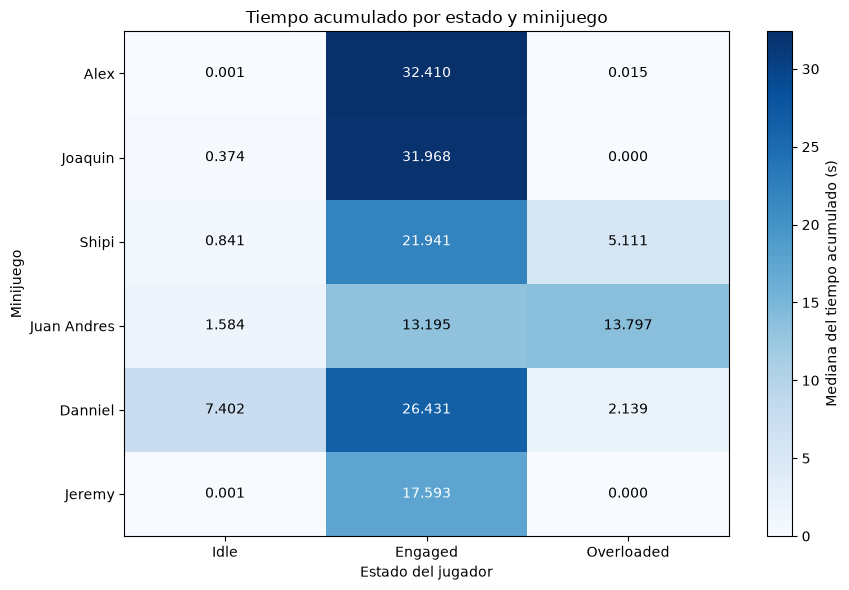
\includegraphics[width=1\textwidth]{imagenes/tiempoAcumuladoPorEstado.png}
    \caption{Mediana del tiempo acumulado, en segundos, que los participantes permanecieron en cada estado durante cada minijuego.}
    \label{fig:graficaTiempoAcumulado}
\end{figure}

\begin{figure}[H]
    \centering
    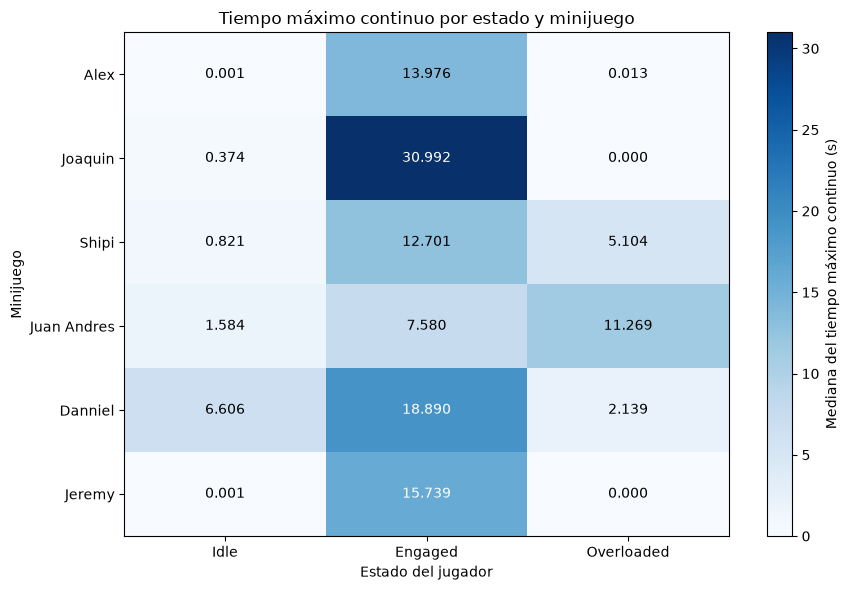
\includegraphics[width=1\textwidth]{imagenes/tiempoContinuoPorEstado.png}
    \caption{Mediana de la duración máxima continua, en segundos, que los participantes permanecieron en cada estado durante cada minijuego.}
    \label{fig:graficaTiempoContinuo}
\end{figure}

\begin{figure}[H]
    \centering
    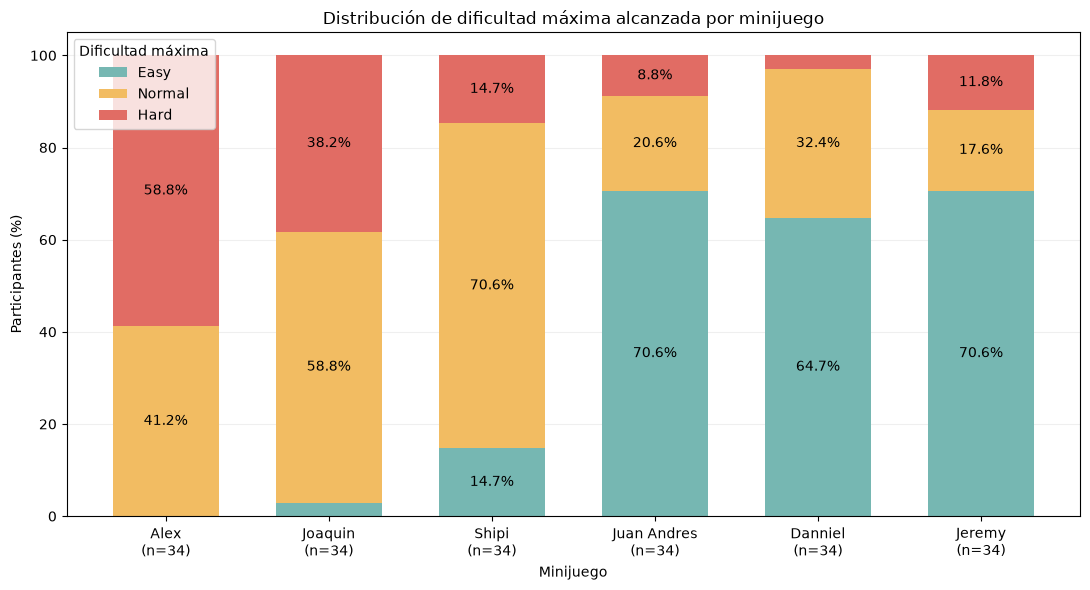
\includegraphics[width=1\textwidth]{imagenes/distribucionMaxDif.png}
    \caption{Distribución porcentual de la dificultad máxima alcanzada por los participantes en cada minijuego.}
    \label{fig:distribucionMaxDif}
\end{figure}

\begin{figure}[H]
    \centering
    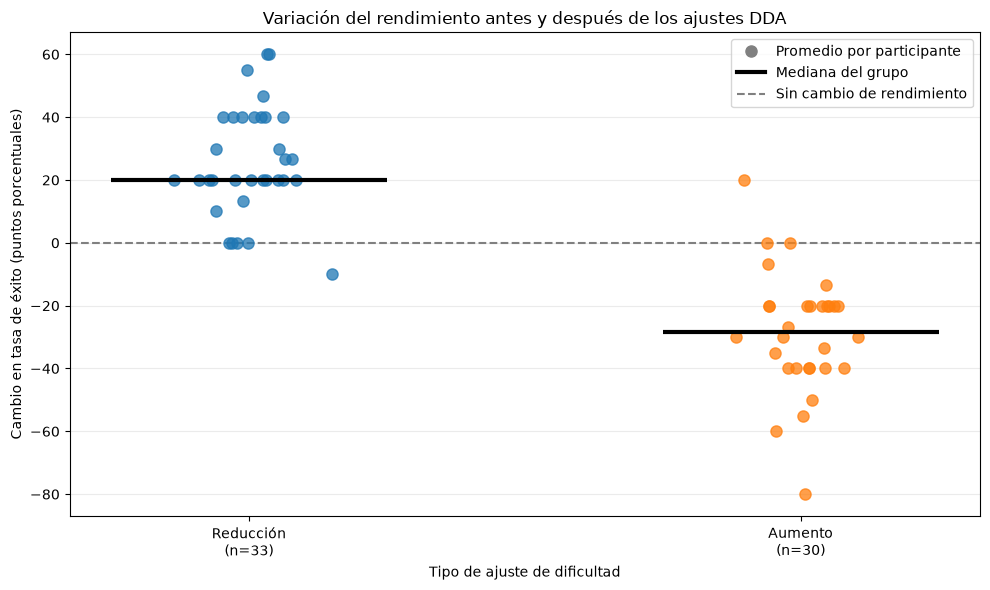
\includegraphics[width=1\textwidth]{imagenes/rendimientoDDA}
    \caption{Gráfica de dispersión del rendimiento de los participantes luego de un aumento y una disminución de dificultad.}
    \label{fig:rendimientoDDA}
\end{figure}

\section{Percepción de dificultad e interacción}
La sección de dificultad e interacción de la encuesta recolecta la 
valoración posterior de cda participante sobre distintos aspectos de la
experiencia. Se consideran las preguntas relacionadas con la atención 
prestada a la canción, la diversión general de la interacción, el nivel
de agobio experimentado, la valoración del propio desempeño y el
minijuego identificado como más frustrante.

\begin{figure}[H]
    \centering
    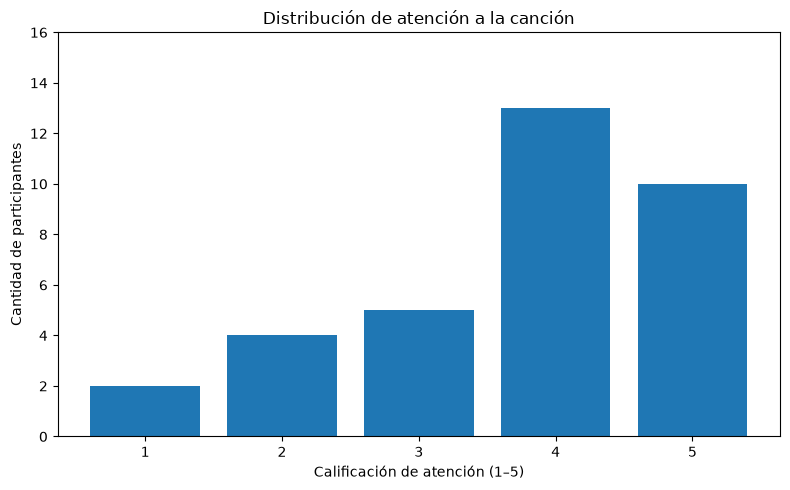
\includegraphics[width=1\textwidth]{imagenes/atencionCancion}
    \caption{Gráfica de distribución de atención a la canción entre participantes.}
    \label{fig:atencionCancion}
\end{figure}

\begin{figure}[H]
    \centering
    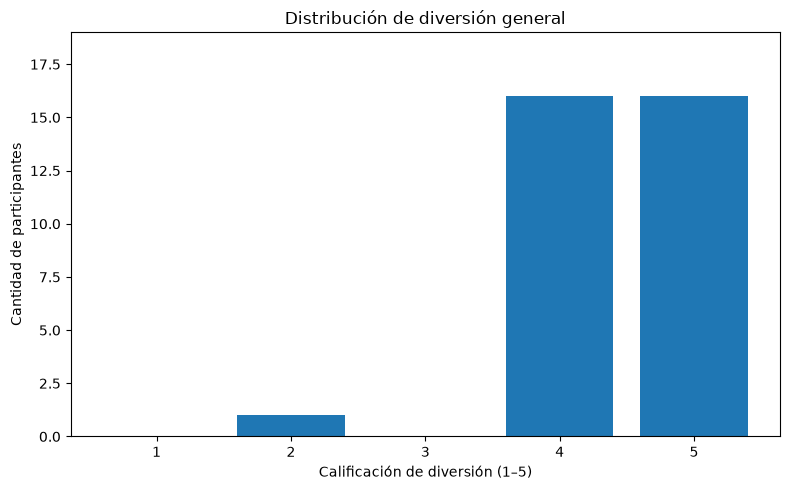
\includegraphics[width=1\textwidth]{imagenes/diversion}
    \caption{Gráfica de distribución de diversión general entre participantes.}
    \label{fig:diversion}
\end{figure}

\begin{figure}[H]
    \centering
    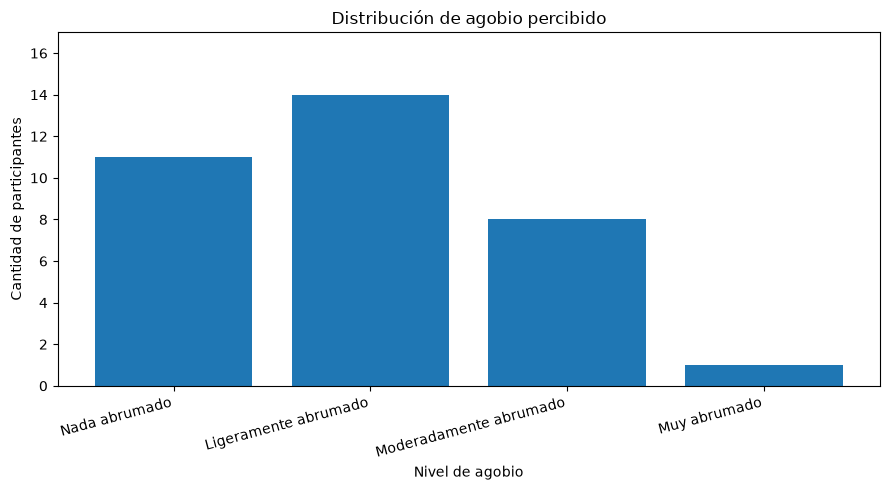
\includegraphics[width=1\textwidth]{imagenes/nivelAgobio}
    \caption{Gráfica de distribución del nivel de agobio entre participantes.}
    \label{fig:nivelAgobio}
\end{figure}

\begin{figure}[H]
    \centering
    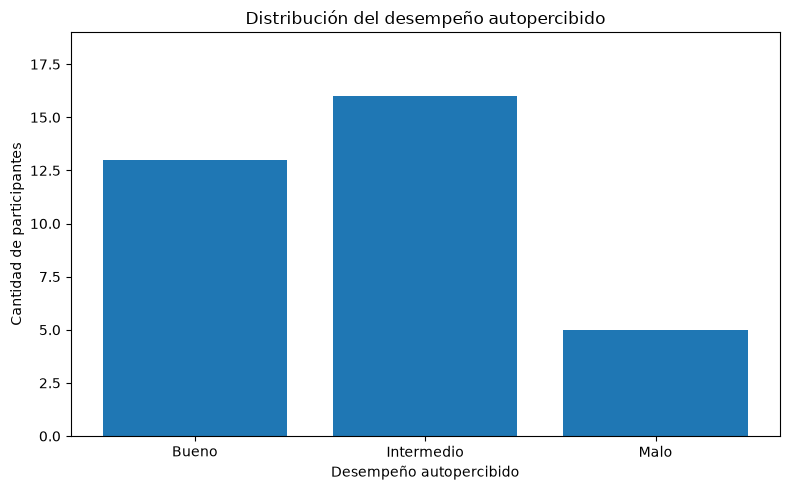
\includegraphics[width=1\textwidth]{imagenes/desempeno}
    \caption{Gráfica de distribución de desempeño autopercibido entre participantes.}
    \label{fig:desempeno}
\end{figure}

\begin{figure}[H]
    \centering
    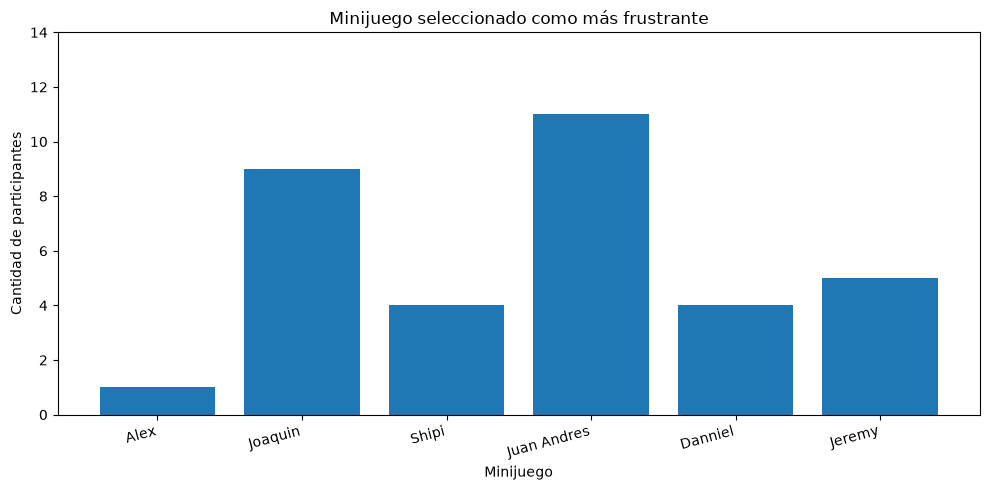
\includegraphics[width=1\textwidth]{imagenes/juegoFrustrante}
    \caption{Gráfica de distribución de minijuegos considerados como los más frustrantes.}
    \label{fig:juegoFrustrante}
\end{figure}

\section{Relación entre telemetría y percepción}
En esta sección se presentan comparaciones entre variables seleccionadas 
de ambas fuentes. Se relacionan, principalmente, el minijuego señalado
como más frustrante con las métricas de desempeño de cada actividad; el
nivel de agobio reportado con la frecuencia de estados 
\textit{Overloaded}; la valoración del desemepeño con la tasa de éxito 
registrada; y la atención presentada a la canción con los indicadores
de desempeño y adaptación obtenidos durante la experiencia.

\begin{figure}[H]
    \centering
    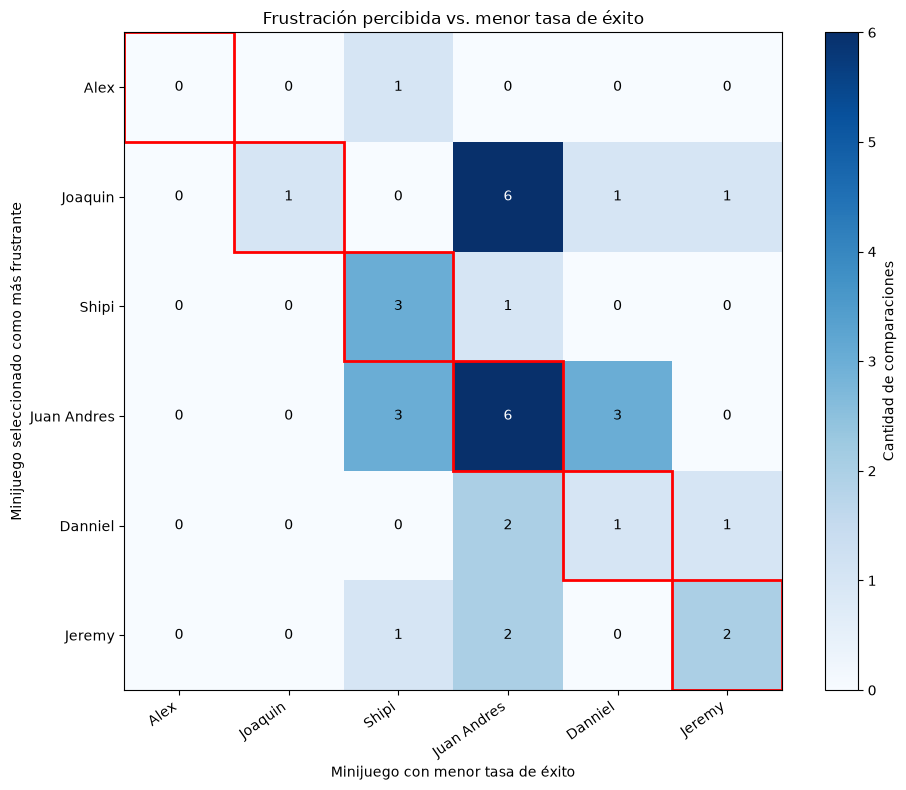
\includegraphics[width=1\textwidth]{imagenes/frustracionVSExito}
    \caption{Mapa de calor de minijuego percibido como más frustrante contra minjuego en el que se tuvo menor tasa de éxito.}
    \label{fig:frustracionVSExito}
\end{figure}

\begin{figure}[H]
    \centering
    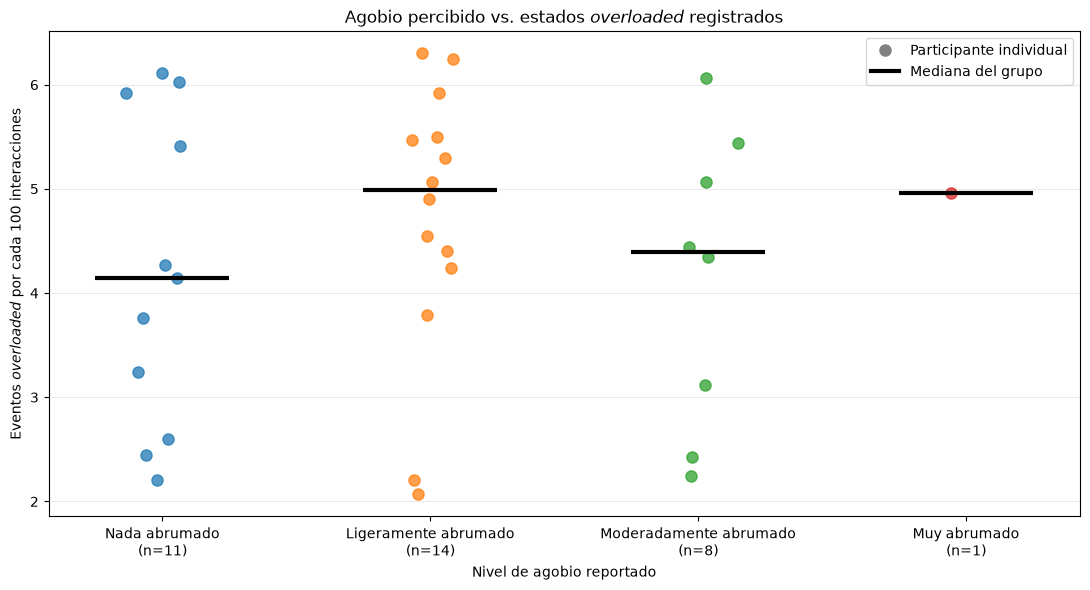
\includegraphics[width=1\textwidth]{imagenes/FrecuenciaOverloaded}
    \caption{Gráfica de dispersión del nivel de agobio percibido contra la frecuencia de estados \textit{overloaded} cada 100 interacciones.}
    \label{fig:FrecuenciaOverloaded}
\end{figure}

% Gráficas de dispersión entre la persepción de frustración de cada 
% minijuego contra 
% a) el tiempo que se estuvo en estado \textit{Idle}, 
% b) el tiempo que se estuvo en estado \textit{Overloaded} y 
% c) el tiempo que se estuvo en estado \textit{Engaged}.
\begin{figure}[H]
    \centering

    \begin{subfigure}[c]{0.48\textwidth}
        \phantomsubcaption
        \label{fig:tiempoIdleVSFrustracion}

        \begin{minipage}{\linewidth}
            \makebox[0.10\linewidth][l]{a)}
            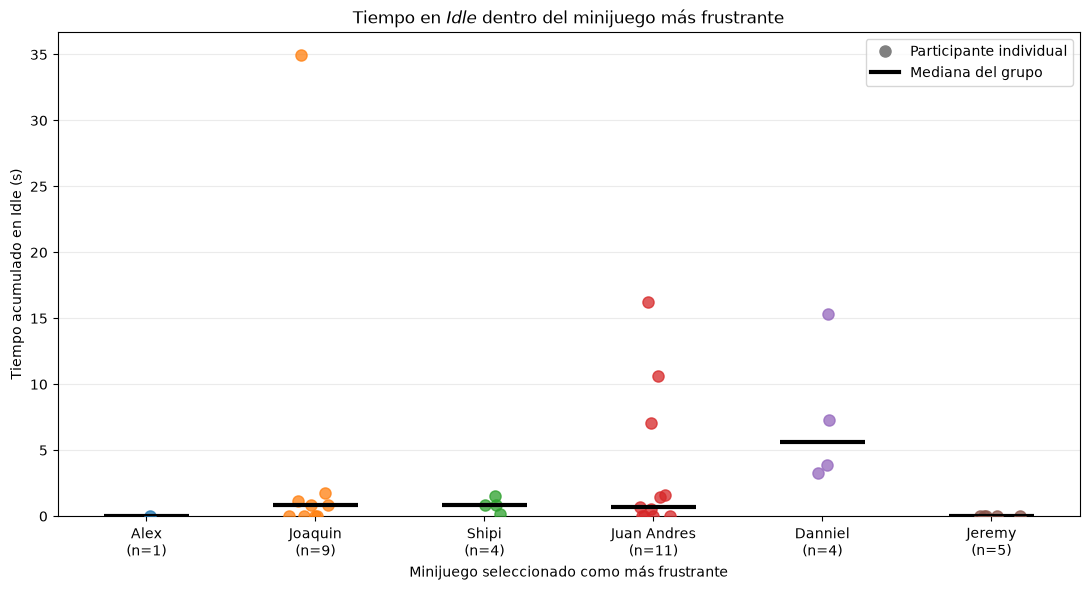
\includegraphics[width=0.88\linewidth]{imagenes/tiempoIdleVSFrustracion.png}
        \end{minipage}
    \end{subfigure}
    \hfill
    
    \begin{subfigure}[c]{0.48\textwidth}
        \phantomsubcaption
        \label{fig:tiempoOverloadedVSFrustracion}

        \begin{minipage}{\linewidth}
            \makebox[0.10\linewidth][l]{b)}
            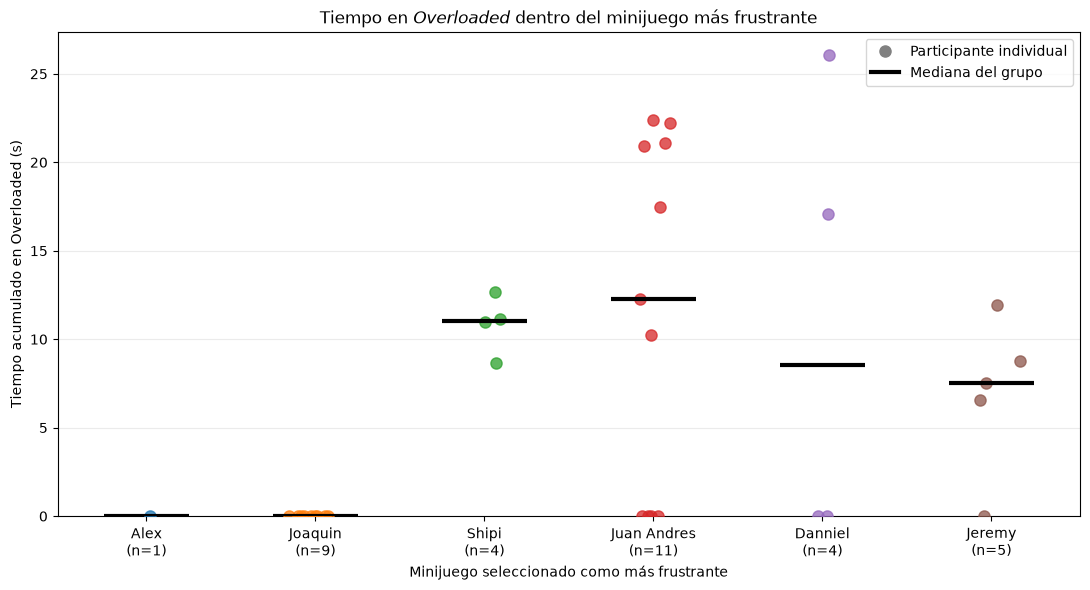
\includegraphics[width=0.88\linewidth]{imagenes/tiempoOverloadedVSFrustracion.png}
        \end{minipage}
    \end{subfigure}
    \hfill

    \begin{subfigure}[c]{0.48\textwidth}
        \phantomsubcaption
        \label{fig:tiempoEngagedVSFrustracion}

        \begin{minipage}{\linewidth}
            \makebox[0.10\linewidth][l]{c)}
            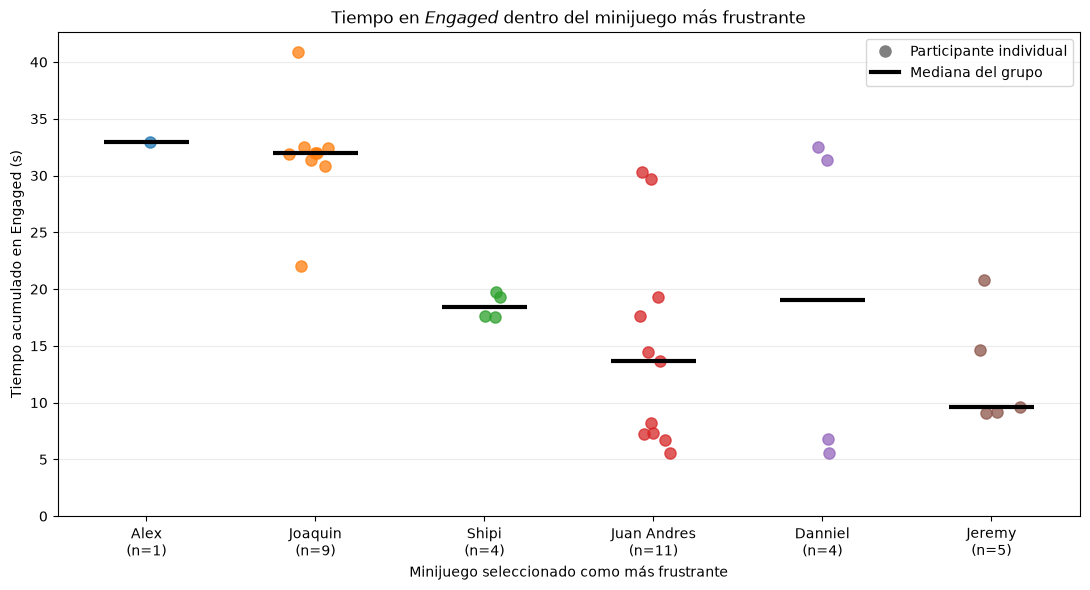
\includegraphics[width=0.88\linewidth]{imagenes/tiempoEngagedVSFrustracion.png}
        \end{minipage}
    \end{subfigure}

    \caption{Gráficas de dispersión entre la percepción de frustración de cada minijuego contra a) el tiempo que se estuvo en estado \textit{Idle}, b) el tiempo que se estuvo en estado \textit{Overloaded} y c) el tiempo que se estuvo en estado \textit{Engaged}.}
    \label{fig:tiempoEstadosVSFrustracion}
\end{figure}

\begin{figure}[H]
    \centering
    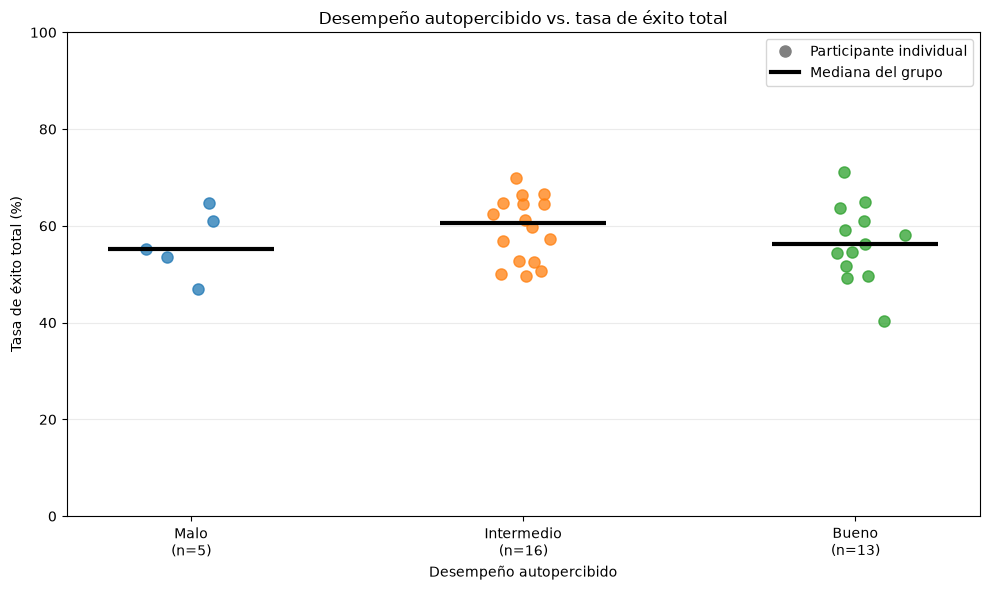
\includegraphics[width=1\textwidth]{imagenes/desempenioVSExito}
    \caption{Gráfica de dispersión del desemepeño autopercibido contra la tasa de éxitos.}
    \label{fig:desempenioVSExito}
\end{figure}

% Gráficas de dispersión de nivel de atención a la canción contra 
% a) estados \textit{overloaded} registrados y 
% b) disminución de la dificultad.
\begin{figure}[H]
    \centering

    \begin{subfigure}[c]{0.48\textwidth}
        \phantomsubcaption
        \label{fig:atencionVSOverload}

        \begin{minipage}{\linewidth}
            \makebox[0.10\linewidth][l]{a)}
            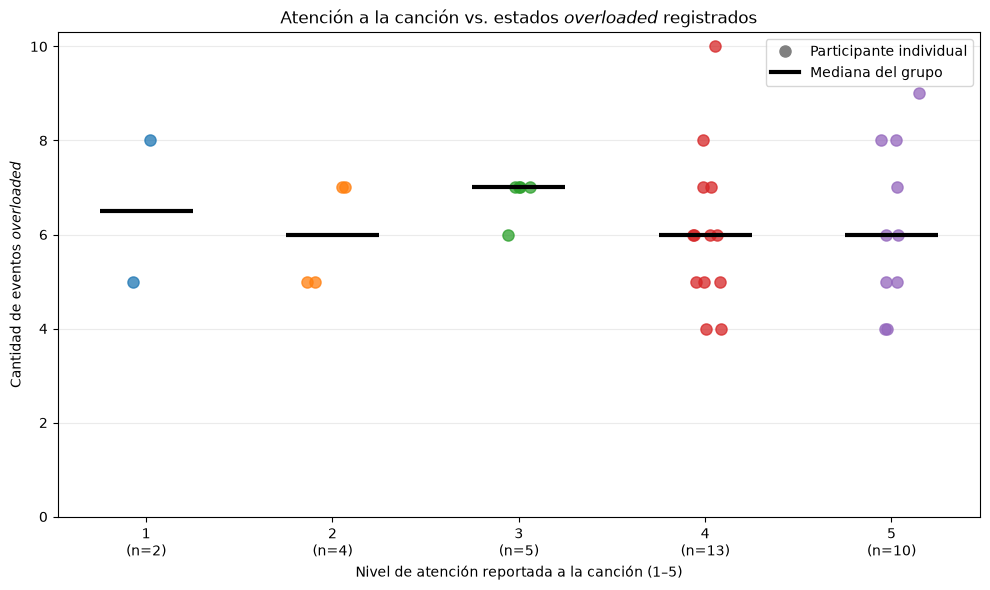
\includegraphics[width=0.88\linewidth]{imagenes/atencionVSOverload}
        \end{minipage}
    \end{subfigure}
    \hfill
    
    \begin{subfigure}[c]{0.48\textwidth}
        \phantomsubcaption
        \label{fig:atencionVSDificultad}

        \begin{minipage}{\linewidth}
            \makebox[0.10\linewidth][l]{b)}
            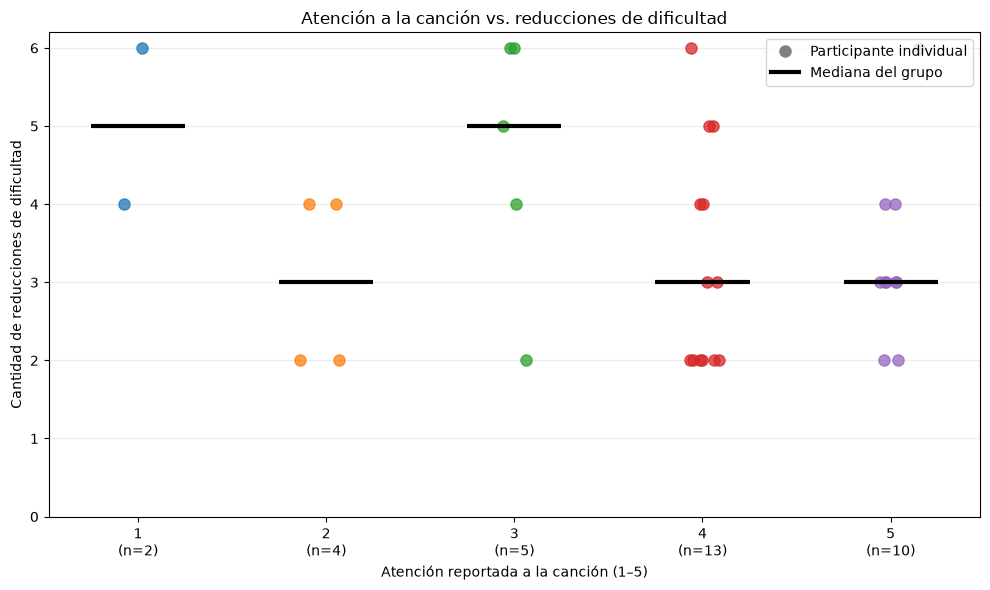
\includegraphics[width=0.88\linewidth]{imagenes/atencionVSDificultad}
        \end{minipage}
    \end{subfigure}

    \caption{Gráficas de dispersión de nivel de atención a la canción contra a) estados \textit{overloaded} registrados y b) disminución de la dificultad.}
    \label{fig:atencionVSDDA}
\end{figure}